\documentclass[]{article}

\usepackage[margin=1.0in]{geometry}
\usepackage[]{graphicx}
\usepackage{listings}

\newcommand\tab[1][1cm]{\hspace*{#1}}

\lstdefinestyle{pythonStyle}{
  language=Python,
  numbers=left,
  stepnumber=1,
  numbersep=10pt,
  tabsize=3,
  showspaces=false,
  showstringspaces=false
}

\begin{document}


\includegraphics[scale=0.1]{res/epoka.png}
\begin{center}
	\begin{large}
		\textbf{
		CEN 350 - Theory of Computation\\
		Louis Alban Ziko\\
		Assignment Report - Recommendation System\\
		}
	\end{large}
\end{center}
\section{Abstract}
\tab This assigment had the topic of a recommendation system. 
We had an algorithm and a search topic randomly assigned to us and had to implement
a recomendation system which would select 10 random websites and search
for keywords related to that topic in those websites. I was assigned Aho Corasick
as my algorithm and programming as my search topic.

\section{Introduction}
\tab \textbf{Aho-Corasick}
is pattern searching algorithm which uses finite automata as it's basis.
It allows for multiple patterns to be searched at once by using a trie(keyword tree)
of all the patterns.
The complexity this algorithm is similar to finite automata. When using 
finite automata the complexity is $\mathcal{O}(n+m)$ where $n$ is the length of the
pattern and $m$ is the length of the text we are searching on. The difference
here is that we have multiple patterns that we go through at the same time so
we need add those up like so $\mathcal{O}(n+m[1]+m[2]+...+m[k])$. So the time
complexity of Aho-Corasick algorithm is $\mathcal{O}(n+\sum_{i=1}^{k} m[i])$.

\section{Dataset}
\tab The dataset I used, i.e. the websites, are included with the code inside the folder
'files'. I selected some which I suspected would lead to a lot a results and some
completely unrelated. The files are in html form. Most of them I download using the 
'wget' command however some wouldn't allow me so I had to copy them using a web browser.

\section{Experiments and Results}
\tab This assigment involved writing a program which would rank 10 websites 
based on how well they relate to a given search topic. I was to use Aho-Corasick
algorithm to find occurences of keywords realted to the search topic.
My search topic was 'programming' so I chose the keywords 'programming', 'algorithm',
'developer' and 'code'.
To write the program I used the python programming language because it
is simple and has quick to write in. I used the python module 'ahocorasick'
for the algorithm implementation. I followed the doc's instructions to create
an automaton and add keywords:

\begin{lstlisting}[style=pythonStyle]
A = ahocorasick.Automaton()
keywords = ["programming", "algorithm", "developer", "code"]
for idx, key in enumerate(keywords):
	A.add_word(key, (idx, key))
A.make_automaton()
\end{lstlisting}


I then used a simple for loop which would run the algorithm through
all the files in the directory:

\begin{lstlisting}[style=pythonStyle]
results = {}
for file_name in os.listdir("files"):
	# set all counters to 0
	counters = {}
	for key in keywords:
		counters[key] = 0
	
	# read file
	with open("files/"+file_name, 'r') as reader:
		# for each occurence of a word increment the corresponding counter
		for end_index, (insert_order, original_value) in A.iter(reader.read()):
			counters[original_value] += 1
	# append the counters to results
	results[file_name] = sum(counters.values())
\end{lstlisting}


All the counts are then in the results variable and so we only need to 
sort them and show them to the console:

\begin{lstlisting}[style=pythonStyle]
# sort the results
result_sorted = dict(sorted(results.items(), key=lambda item: item[1],
	reverse=True))

# show the results
print("web_page\t|\tcount")
print("-" * 30)
for key in result_sorted:
	print("{0}\t|\t{1}".format(key, result_sorted[key]))
\end{lstlisting}

Here is what the result looks like:\\
\\
\begin{center}
	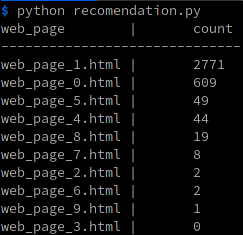
\includegraphics[scale=0.7]{res/recomendation.png}
\end{center}


\end{document}